\chapter{Theory}\label{cha:theory}

\section{The Standard Model of Particle Physics}\label{sec:theory:sm}


\section{Hadronic scattering and parton model}\label{sub:theory:hadronscattering}

Today Higgs bosons can only be investigated at hadron colliders.
A hadron is no fundamental particles, it is a combination of several quarks bound by the strong force.
In the following a two-particle scattering
\begin{equation}
    1 + 2 \to 3 + 4
\end{equation}
is discussed.
The four-momenta of the particles are denoted by $p_i$ with $i = 1,\ldots,4$.

The structure of hadrons can be described with the structure functions $W_1(Q^2, \nu)$ and $W_2(Q^2, \nu)$,
which depend on the squared four-momentum transfer
\begin{equation}
    Q^2 = -q^2 = - (p_1 - p_3)^2
\end{equation}
and the transferred energy $\nu = E' - E$.
The structure functions are measured in deep inelastic electron--nucleon scattering experiments.
The cross-section for those scatterings can be written as~\cite{drell64, bjo:scaling}
\begin{equation}
    \frac{\dif \sigma}{\dif\Omega \dif E'} = \frac{\alpha^2}{4 E^2 \sin^4 \frac{\theta}{2}}
    \left[ W_2(Q^2, \nu) \cos^2 \frac{\theta}{2} + 2 W_1(Q^2, \nu) \sin^2 \frac{\theta}{2} \right ],
\end{equation}
with the fine-structure constant $\alpha$, the energies $E$ and $E'$ of the electron before and after the scattering,
and the scattering angle $\theta$, the angle between the electron beam, and the scattered electron.

For large energies the quantities $Q^2$ and $\nu$ are not longer independent of each other.
$W_1$ and $\nu W_2$ only depend on a single variable, the \emph{Bjorken scaling variable}, $x$:
\begin{equation}
    x = \frac{Q^2}{2 M \nu} \,,
\end{equation}
where $M$ is the mass of the nucleon.
In the asymptotic limit the structure of hadrons can be described with the structure functions $F_1(x)$ and $F_2(x)$,
\begin{equation}
    \begin{split}
        \lim_{Q^2, \nu \to \infty} W_1(Q^2, \nu) &= F_1(x) \,, \\
        \lim_{Q^2, \nu \to \infty} \nu W_2(Q^2, \nu) &= F_2(x) \,.
    \end{split}
\end{equation}
This phenomenon was discovered experimentally and is called \emph{Bjorken scaling} after its discoverer, J.\ D.\ Bjorken~\cite{bjo:scaling}.

Richard Feynman and E. A. Paschos proposed a descriptive model for the structure of the proton, the so called
\emph{parton model}~\cite{feyn69,bjo:epscattering}.
According to this model the proton can be described as an accumulation of free, charged, point-like particles, the \emph{partons}.
This view makes only sense in the \emph{infinite momentum frame}, a reference frame where the proton has infinite
momentum.\footnote{The center-of-mass frame of the colliding particle and the proton is a good approximation
for such a frame at high energies~\cite{bjo:epscattering}.}
In this frame the transverse momenta and masses of the partons are negligible.
The four-momentum $p_i$ of a parton $i$ is a fraction $x_i \ (0 \leq x_i \leq 1)$ of the total four-momentum $p$ of the proton:
\begin{equation}
    p_i = x_i p\,, \qquad\text{with } \sum_i x_i = 1\,.
\end{equation}
The fraction $x_i$ can be identified with the Bjorken scaling variable~\cite{bjo:epscattering}: $x$ is the momentum fraction of the parton
by which the lepton has been scattered.

The generalized probability density to find a parton $i$ with the longitudinal momentum fraction $x_i$ is defined as the
parton distribution function (PDF) $f_i(x, M_\text{F}^2)$.
$M_\text{F}$ is the factorization scale, a distinction between hard and soft scattering.
Since PDFs cannot be calculated within perturbation theory, they are determined with the help of fits to experimental data.
The DGLAP evolution equations (Dokshitzer, Gribov, Lipatov, Altarelli, Parisi)~\cite{dglap:d, dglap:gl, dglap:ap}
can be used to evolve the experimentally provided PDFs to other factorization scales, which may not be accessible by experiments.

\cref{fig:theory:pdfs} displays the PDFs of different partons in protons.
The PDFs of the up and down quarks are not equal to the PDFs of their antiquarks.
This is caused by the internal structure of the proton.
There are three \emph{valence quarks}, two up and one down quark, which together determine the quantum numbers of the proton.
These quarks constantly exchange gluons, which may produce a temporary quark--antiquark pair, the so-called \emph{sea quarks}.
Because the sea quarks only exists in pairs, the probability to find an up or down quark in a proton is larger than finding an
antiup or antidown quark.
\begin{figure}[htb]
	\centering
	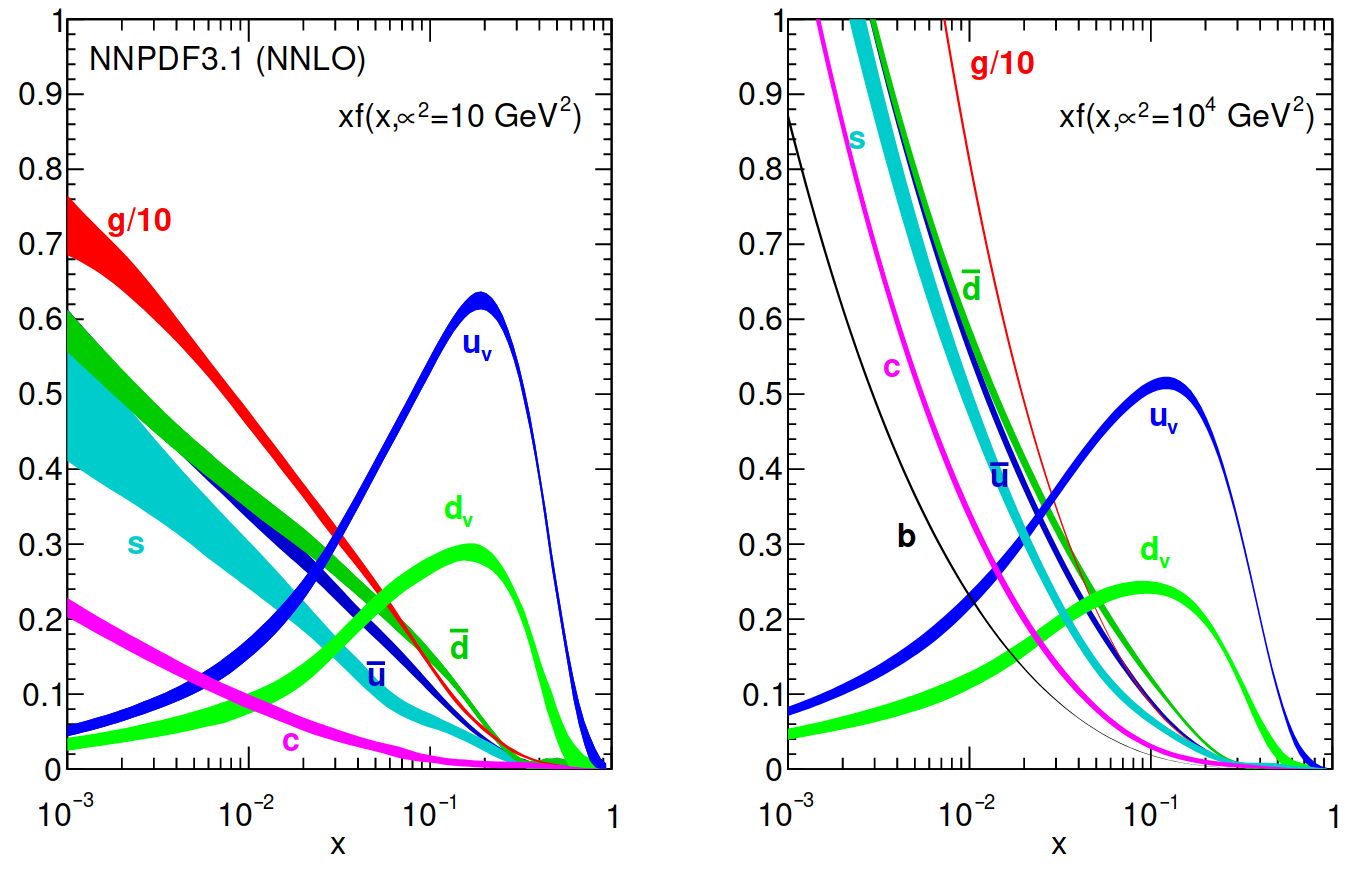
\includegraphics[width=0.7\textwidth]{./figures/theory/nnpdf.png}
	\caption{PDFs for different partons as a function of the Bjorken scaling variable $x$
             for two different factorization scales $Q^2 = \SI{10}{\GeV\squared}$ and $Q^2 = \SI{e4}{\GeV\squared}$.
			 The PDF set is NNPDF3.1 (NNLO)~\cite{nnpdf3.1}.}\label{fig:theory:pdfs}
\end{figure}
Another property of quark partons is indicated: It is less probable to find a quark with a higher mass.
The probability to find a photon is highly repressed, in contrast to the gluon PDF, which has the highest value for small $x$.

A dependency on the factorization scale $Q^2$ is recognizable.
The predicted independence of the PDFs from $Q^2$ only holds approximately for certain values.
But the parton model of Feynman still can be used as a foundation to describe inelastic scattering.
There are more complicated models like the \emph{QCD-improved parton model}~\cite{col98}, where
partons are allowed to interact between each other by exchanging gluons.

\todo{Shorten/rephrase section}

\section{The Higgs Boson}\label{sec:theory:higgs}

\subsection{Higgs Boson Production in Proton--Proton Collisions}
\label{sub:theory:higgs:production}

In proton--proton collisions at the LHC the parton model as described above can be applied.
To calculate the cross-section of the production of a particle $X$ in proton--proton collisions the
cross-section at parton level $\hat{\sigma}_{ij\to X}$ has to be weighted with the PDFs and all
possible momentum fractions need to be considered, as prescribed by the factorization theorem~\cite{DRELL1971578}.
Mathematically speaking this is a convolution of the PDFs with the partonic cross-section,
\begin{equation}
    \sigma_{ij\to X} = \int_{0}^{1} \dif x_i \int_{0}^{1} \dif x_j \,
    f_i \left( x_i \right ) f_j \left( x_j \right ) \hat{\sigma}_{ij\to X} \,.
\end{equation}
The general expression of the partonic cross-section is~\cite{griffiths}
\begin{equation}
    \hat{\sigma}_{ij\to X} = \frac{1}{j} \int \matrixm \left(ij \to X \right) \dif \Phi \,,
\end{equation}
with the matrix element $\matrixm$ which describes the transition probability of the initial state $ij$ to the final state $X$, the
particle flux $j$, and the phase-space factor $\dif \Phi$ depending on the kinematics of the collision.
\\[\baselineskip]
The Higgs boson can be produced in multiple ways, which vary in cross-section and phenomenology.
In \cref{fig:theory:higgs:production} the leading order (LO) Feynman diagrams are shown for the dominant production modes
at the LHC\@.

\begin{figure}[htb]
    \centering
    \begin{subfigure}[t]{0.302\textwidth}
        \includegraphics[width=\textwidth]{feynman/h_ggf.pdf}
        \caption{gluon--gluon fusion}\label{fig:theory:higgs:ggf}
    \end{subfigure}
    \begin{subfigure}[t]{0.201\textwidth}
        \captionsetup{justification=raggedright}
        \includegraphics[width=\textwidth]{feynman/h_vbf.pdf}
        \caption{vector boson fusion}\label{fig:theory:higgs:vbf}
    \end{subfigure}
    \begin{subfigure}[t]{0.201\textwidth}
        \includegraphics[width=\textwidth]{feynman/h_strahl.pdf}
        \caption{Higgs-Strahlung}\label{fig:theory:higgs:vbf}
    \end{subfigure}
    \begin{subfigure}[t]{0.246\textwidth}
        \captionsetup{justification=raggedright}
        \includegraphics[width=\textwidth]{feynman/h_top.pdf}
        \caption{associated \mbox{production} with top-quarks}\label{fig:theory:higgs:vbf}
    \end{subfigure}
    \caption{Feynman diagrams of the most important production modes of the Higgs boson at the LHC\@. The cross-section
             decreases from left to right.}\label{fig:theory:higgs:production}
\end{figure}

\subsection{Decay Modes of the Higgs Boson}
\label{sub:theory:higgs:decay}

\section{Measurements of the Higgs Boson at the LHC}
\label{sec:theory:measurements}


